% Auto-generated by final_report/build_report.py.
        \documentclass[letterpaper]{article}
        \usepackage[draft]{aaai2026}
        \usepackage{times}
        \usepackage{helvet}
        \usepackage{courier}
        \usepackage[hyphens]{url}
        \usepackage{graphicx}
        \urlstyle{rm}
        \def\UrlFont{\rm}
        \usepackage{natbib}
        \usepackage{caption}
        \frenchspacing
        \setlength{\pdfpagewidth}{8.5in}
        \setlength{\pdfpageheight}{11in}
        \providecommand{\pdfinfo}[1]{}
        \pdfinfo{/TemplateVersion (2026.1)}
        \setcounter{secnumdepth}{0}

        \title{Complementary Member-Level Regularization for TabM on TabReD}
        \author{Prithvi Nishal (G2504965H), Pentamsetty Sai Harshita (G2503340A),\\
        Nath Simerjit Kaur (G2507742D), Abhipray Chavan (G2504327J)}
        \affiliations{Nanyang Technological University}

        \begin{document}
        \maketitle

        \begin{abstract}
        TabM is a recent tabular deep learning baseline built around parameter-efficient ensembling. We test four concrete member-level questions on five TabReD datasets: whether TabM benefits from more adapter capacity, flatter adapter optima, fixed member-level feature diversity, or structured adapter saliency. Our implementation keeps the official TabM-PLR per-dataset pipeline and adds four corresponding modifications: rank-adaptive low-rank adapters (RLA), adapter-focused sharpness-aware optimization (ESAM), member-fixed feature bagging (MFB), and teacher-importance distillation over adapter feature saliency (CF-FISD). Individually, no module dominates all datasets. Under validation-selected matched inference, a per-dataset set of compatible module combinations improves over the corresponding TabM-PLR baseline on all five datasets. The result is intentionally scoped: default mean-inference TabM-PLR remains better on some datasets, so the main finding is complementarity under matched inference, not a replacement for the paper baseline.
        \end{abstract}

        \section{Introduction}
        Tabular data remains a difficult setting for deep learning because tree models and well-tuned MLPs are hard baselines. TabM~\citep{gorishniy2025tabm} addresses this by producing multiple predictions from one parameter-efficient MLP ensemble based on BatchEnsemble-style member adapters~\citep{wen2020batchensemble}. The paper shows that the members are weak individually but useful collectively; this makes the internal member structure a concrete part of the model to test. Our project asks whether that structure can be improved by shaping capacity, optimization, feature exposure, and feature saliency at the member level.

        We use the project option of improving a post-2019 conference paper with its public codebase. The target paper is TabM, an ICLR 2025 paper, and the benchmark is TabReD~\citep{rubachev2024tabred}, a tabular benchmark with realistic splits and heterogeneous tasks. PLR in this report means the PiecewiseLinearEmbeddings numerical embedding setup used by the TabM paper configs. The contribution is not a new dataset or a lowered baseline. Instead, the report evaluates four modifications on top of the same TabM-PLR per-dataset configs.

        The main result has a narrow scope. The validation-selected combined method improves over matched-inference TabM-PLR on all five selected TabReD datasets. This is not the same as beating the default mean-inference TabM baseline everywhere. We report both comparisons to avoid artificially lowering the baseline.

        \section{Relationship to the TabM Paper}
        The paper comparison in this report is against the official TabM-PLR implementation path. We do not replace TabM with a simplified MLP, retune the baseline downward, or change the per-dataset data policies. The official paper pipeline uses TabM with PiecewiseLinearEmbeddings, tuned optimizer settings, dataset-specific policies, and $k=32$ members for these TabReD-style experiments. Our code keeps that pipeline and adds module flags around the member adapters.

        Table~\ref{tab:paper_alignment} summarizes the alignment. The important distinction is that the released paper used a broader evaluation budget, while our final confirmation run uses three seeds for every final row. Therefore, our result should be read as a controlled project reproduction and extension of the TabM paper configuration, not as a claim that we have replaced the full published leaderboard.

        \begin{table}[!htbp]
\centering
\small
\begin{tabular}{p{0.23\columnwidth}p{0.65\columnwidth}}
\hline
Item & Protocol \\
\hline
Paper target & TabM, ICLR 2025 \\
Baseline & Official per-dataset TabM-PLR configs \\
Data & Five available TabReD datasets \\
Metrics & RMSE for regression, AUROC for binary tasks \\
Kept fixed & Preprocessing, data policy, tuned optimizer, $k$, patience \\
Changed & Only module-specific adapter/loss/masking flags \\
Selection & Validation-only; report matched and default-mean baselines \\
\hline
\end{tabular}
\caption{Comparison protocol against the TabM paper implementation. The report compares against a reproduced paper-config TabM-PLR baseline, not a simplified local baseline.}
\label{tab:paper_alignment}
\end{table}

        \begin{figure}[!htbp]
        \centering
        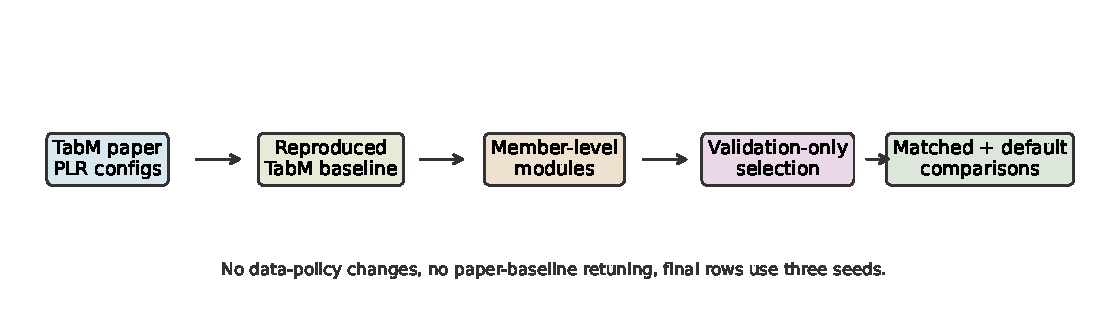
\includegraphics[width=\columnwidth]{fig_protocol_bridge.pdf}
        \caption{How the experiment connects the TabM paper implementation to our modified system.}
        \label{fig:protocol}
        \end{figure}

        \section{Methods}
        \textbf{TabM baseline.} TabM trains an MLP backbone that emits $k$ member predictions using parameter-efficient per-member multiplicative adapters. At inference, the default prediction is the mean over members, while best-head and greedy-head modes select heads or subsets using validation scores. Our baseline is the official TabM-PLR configuration for each dataset: tuned optimizer, architecture, embeddings, data policy, $k$, patience, and dataset-specific preprocessing are preserved.

        \textbf{RLA.} Rank-adaptive low-rank adapters generalize the rank-1 member adapter path to multiple low-rank paths while preserving the original base path. The intended effect is to increase member-specific capacity without turning TabM into a fully separate ensemble. Empirically, this helped most when the additional paths were small and base-preserving; aggressive extra capacity could overfit or destabilize the already competitive PLR baseline.

        \textbf{ESAM.} ESAM applies sharpness-aware optimization~\citep{foret2021sam} to the member-specific adapter parameters. This targets per-member overfitting and encourages flatter adapter solutions while leaving the common TabM training pipeline intact. We restrict the perturbation to adapter-heavy parameter groups so that ESAM changes the ensemble members more than the shared backbone.

        \textbf{MFB.} Member-fixed feature bagging assigns deterministic feature masks to TabM members. This directly increases input-level diversity among members while retaining the shared backbone. Unlike stochastic dropout, the masks are member-specific and stable, so each member learns a consistent view of the feature space.

        \textbf{CF-FISD.} CF-FISD aligns member adapter feature saliency with feature-importance profiles from external tabular teachers. The implemented loss groups TabM members by teacher family and penalizes mismatch between adapter saliency and teacher feature importance. This gives a structured signal to adapter weights without feeding teacher predictions into the final model.

        These four methods target different questions about TabM's members: adapter capacity, optimization sharpness, input-level diversity, and feature-saliency alignment. The combined system is validation-selected per dataset from compatible module combinations. It is therefore a validation-selected model family, not a single fixed all-four architecture.

        Conceptually, the modules act at four different points of the same TabM member pipeline. If $f_i(x)$ is the prediction of member $i$, RLA changes the capacity of the member adapter producing $f_i$, ESAM changes the local optimization landscape of those adapter parameters, MFB changes the member-specific input view of $x$, and CF-FISD regularizes the adapter saliency pattern. The design goal is complementarity rather than one universal knob.

        \begin{figure}[!htbp]
        \centering
        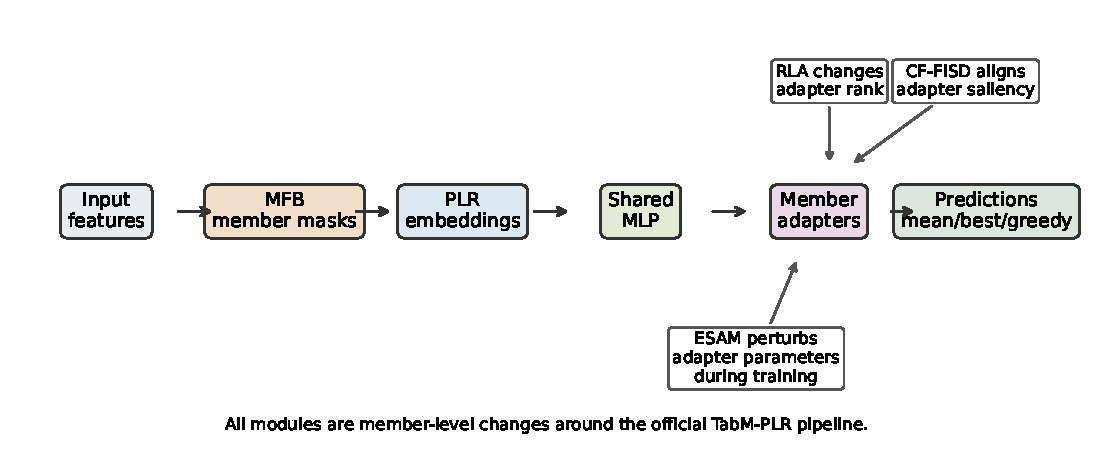
\includegraphics[width=\columnwidth]{fig_method_diagram.pdf}
        \caption{Where each modification acts in the TabM-PLR pipeline. The diagram is intentionally limited to the mechanisms used in the final integrated code.}
        \label{fig:method}
        \end{figure}

        \section{Implementation Details}
        The integrated code keeps a single TabM training entry point and exposes each modification through explicit configuration fields. This is important because the baseline and modified runs share the same data loader, metric computation, early stopping, and evaluation code. When all module flags are disabled, the run path is the paper-config TabM-PLR baseline. When a module is enabled, the change is localized to adapter construction, optimizer behavior, feature masking, or the auxiliary CF-FISD loss.

        RLA is implemented in the adapter construction path. The base-preserving variants keep the original rank-1 behavior as one path and add low-rank residual paths with small initialization noise. This design was chosen after early sweeps showed that simply increasing adapter rank could hurt on saturated datasets. ESAM is implemented in the training step rather than as a separate model: it perturbs selected adapter parameters, evaluates the sharpness-aware objective, and restores the parameters before the optimizer update. MFB is implemented before the shared MLP blocks by applying member-indexed masks over feature groups. CF-FISD is implemented as an auxiliary loss over the first adapter saliency, with teacher feature-importance vectors loaded from the bundled teacher artifacts.

        The combined rows are not a single all-modules-on run. They are validation-selected compositions from compatible module subsets. This matters because some modules conflict on specific datasets: for example, feature bagging can help one dataset while hurting another, and extra adapter capacity can be useful for one target but noisy for another. The per-dataset selection rule is therefore part of the method. The report names this explicitly so that the reader does not confuse the final 5/5 row with a single fixed architecture.

        The implementation also records enough metadata to audit the comparisons. Each final row contains the selected source variant, metric direction, inference mode, matched baseline mean, default mean baseline, final mean and standard deviation, and seed count. Without those fields, the same numerical table could accidentally compare a best-head result to a mean-inference baseline, which would overstate the result. The final report is generated from that CSV rather than from manually typed values.

        \section{Experimental Protocol}
        We evaluate five TabReD datasets: sberbank-housing, ecom-offers, homesite-insurance, cooking-time, and delivery-eta. Regression datasets use RMSE, where lower is better. Binary classification datasets use AUROC, where higher is better. Using both metrics is expected because TabReD mixes regression and binary classification tasks.

        Every final reported row uses three seeds. Model selection is performed using validation metrics only. For a fair comparison with validation-selected inference modes, the main delta compares each selected variant to TabM-PLR evaluated with the same inference mode. We also report the delta against the default mean-inference baseline, because it is the most conservative view of whether the method improves the usual TabM deployment. The final matrix contains 30 rows: one TabM-PLR baseline plus five method rows for each dataset.

        The protocol deliberately separates three questions. First, does an individual module help under a matched inference mode? Second, do the modules help different datasets, making them complementary? Third, does a validation-selected combined method improve over a correspondingly selected TabM baseline? This separation is necessary because a single sign-based table can hide the fact that an improvement depends on the inference mode.

        \section{Ablation Study}
        We ran more ablations than can fit as raw tables in the main report. The main paper therefore reports ablation families, not every single failed setting. This is deliberate: the reader should see the logic of the search and the evidence behind the final choices without having to parse hundreds of near-duplicate runs. Table~\ref{tab:ablations} lists the ablations that changed the final interpretation.

        \begin{table}[!htbp]
\centering
\footnotesize
\setlength{\tabcolsep}{2pt}
\begin{tabular}{p{0.27\columnwidth}p{0.65\columnwidth}}
\hline
Ablation & What it showed \\
\hline
Baseline fidelity & Paper-config TabM-PLR is the reference row; we do not lower or simplify the baseline. \\
RLA capacity & Rank, initialization, noise, freeze, and inference sweeps show capacity helps Sb. and Dl., but not every dataset. \\
ESAM sharpness & Rho and adapter-only sweeps show ESAM helps Ec., Hs., and Ck. \\
MFB diversity & Member mask and keep-rate sweeps show feature diversity helps Ec., Ck., and Dl. \\
CF-FISD saliency & Teacher-alignment and lambda sweeps help Sb. and Hs.; Dl. is neutral under matched inference. \\
Combined subsets & Compatible module subsets are validation-selected per dataset; the selected combinations improve 5/5 matched. \\
Inference audit & Mean, best-head, and greedy-head baselines are compared separately to avoid inflated claims. \\
Rejected screens & Auxiliary objectives and k-scaling screens are not used in the final selected rows. \\
\hline
\end{tabular}
\caption{Ablation coverage in the main report. The raw grids contain more individual trials; the table lists the ablation families that affect the final conclusion.}
\label{tab:ablations}
\end{table}

        The ablations answer a specific question rather than just searching for a better number. RLA tests whether TabM's rank-1 member adapter is a capacity bottleneck. ESAM tests whether the member adapters overfit sharply. MFB tests whether fixed member-specific feature exposure improves diversity. CF-FISD tests whether teacher feature-importance structure can guide adapter saliency. The combined-subset ablation then tests whether the datasets helped by each module are complementary. This avoids the weak argument ``we tried many things and one worked''; the evidence is organized around concrete properties of TabM's member ensemble.

        \section{Results}
        Table~\ref{tab:combined} shows the final validation-selected combined method. The selected combinations differ by dataset: RLA+MFB+CF-FISD for sberbank-housing, MFB+CF-FISD for ecom-offers and homesite-insurance, RLA+ESAM for cooking-time, and RLA+CF-FISD for delivery-eta. These selected combinations improve all five datasets under matched inference: +2.047\% on sberbank-housing, +0.806\% AUROC on ecom-offers, +0.018\% AUROC on homesite-insurance, +0.021\% on cooking-time, and +0.423\% on delivery-eta. The wins are small on several datasets, which is expected because TabM-PLR is already a competitive baseline.

        \begin{table}[!htbp]
\centering
\setlength{\tabcolsep}{2pt}
\footnotesize
\begin{tabular}{lllccc}
\hline
Data & Combo & Inf. & $\Delta_m$ & $\Delta_\mu$ & S \\
\hline
Sb/RMSE & R+M+CF & best & +2.047\% & -4.548\% & W \\
Ec/AUROC & M+CF & greedy & +0.806\% & +2.568\% & C \\
Hs/AUROC & M+CF & greedy & +0.018\% & +0.037\% & W \\
Ck/RMSE & R+E & greedy & +0.021\% & +0.074\% & W \\
Dl/RMSE & R+CF & best & +0.423\% & -0.747\% & C \\
\hline
\end{tabular}
\caption{Final validation-selected combined results. Data includes the metric. Combo abbreviations: R = RLA, E = ESAM, M = MFB, CF = CF-FISD. $\Delta_m$ is matched-inference improvement; $\Delta_\mu$ is improvement over default mean-inference TabM-PLR. S: C = clear win, W = weak win. Mean and standard deviation values are in the released CSV artifact.}
\label{tab:combined}
\end{table}

        Table~\ref{tab:baseline_values} makes the paper-config comparison explicit. The first numeric baseline is the reproduced default mean-inference TabM-PLR row, which corresponds to the usual paper deployment mode. The matched baseline is the same TabM-PLR model evaluated with the selected inference mode. This distinction matters because the matched baseline can be weaker or stronger than default mean inference depending on the dataset.

        \begin{table}[!htbp]
\centering
\footnotesize
\setlength{\tabcolsep}{2pt}
\begin{tabular}{lcccc}
\hline
Data & Default & Matched & Ours & $\Delta_m$ \\
\hline
Sb/RMSE & 0.2344 & 0.2502 & 0.2451 & +2.047\% \\
Ec/AUROC & 0.5901 & 0.6004 & 0.6052 & +0.806\% \\
Hs/AUROC & 0.9625 & 0.9627 & 0.9628 & +0.018\% \\
Ck/RMSE & 0.4804 & 0.4801 & 0.4800 & +0.021\% \\
Dl/RMSE & 0.5502 & 0.5567 & 0.5543 & +0.423\% \\
\hline
\end{tabular}
\caption{Paper-config baseline comparison. Default is the reproduced default mean-inference TabM-PLR baseline. Matched is TabM-PLR under the same selected inference mode as Ours.}
\label{tab:baseline_values}
\end{table}

        The default mean comparison is more conservative. It remains positive on ecom-offers, homesite-insurance, and cooking-time, but negative on sberbank-housing and delivery-eta. This means the safe claim is not that the method improves over default TabM in every deployment mode. The safe claim is that validation-selected module composition improves the corresponding validation-selected TabM inference baseline on every dataset.

        \begin{figure}[!htbp]
        \centering
        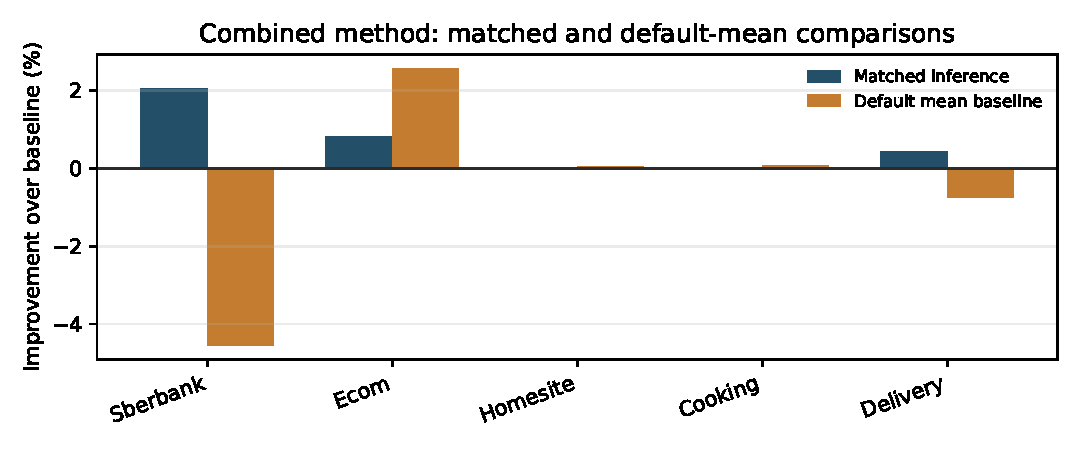
\includegraphics[width=\columnwidth]{fig_combined_comparison.pdf}
        \caption{Combined method improvements under the matched-inference protocol and the conservative default mean-inference comparison.}
        \label{fig:combined}
        \end{figure}

        Figure~\ref{fig:combined} is the central paper-baseline comparison. The blue bars compare the selected combined method to the TabM-PLR baseline under the same inference mode. The orange bars compare the same selected method to the default mean-inference TabM-PLR baseline. This is why the paper claim is not overstated: sberbank-housing and delivery-eta are still worse than default mean TabM, even though they are positive under matched best-head inference.

        \begin{figure}[!htbp]
        \centering
        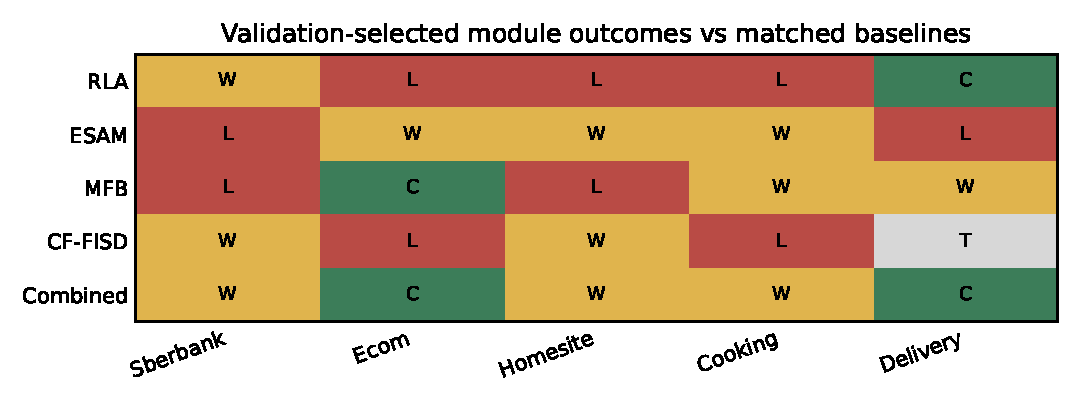
\includegraphics[width=\columnwidth]{fig_module_heatmap.pdf}
        \caption{Outcome heatmap for individual modules and the final combined system.}
        \label{fig:heatmap}
        \end{figure}

        \begin{table}[!htbp]
\centering
\small
\begin{tabular}{lccccc}
\hline
Method & Sb. & Ec. & Hs. & Ck. & Dl. \\
\hline
RLA & W & L & L & L & C \\
ESAM & L & W & W & W & L \\
MFB & L & C & L & W & W \\
CF-FISD & W & L & W & L & T \\
Combined & W & C & W & W & C \\
\hline
\end{tabular}
\caption{Matched-baseline outcome matrix. C = clear win, W = weak win, T = tie, L = loss. Dataset abbreviations follow Table~\ref{tab:combined}.}
\label{tab:matrix}
\end{table}

        Table~\ref{tab:matrix} and Figure~\ref{fig:heatmap} show why combining modules matters. RLA helps sberbank-housing and delivery-eta, ESAM helps ecom-offers, homesite-insurance, and cooking-time, MFB helps ecom-offers, cooking-time, and delivery-eta, and CF-FISD helps sberbank-housing and homesite-insurance. No individual modification is universal, but the error patterns are complementary.

        \begin{figure}[!htbp]
        \centering
        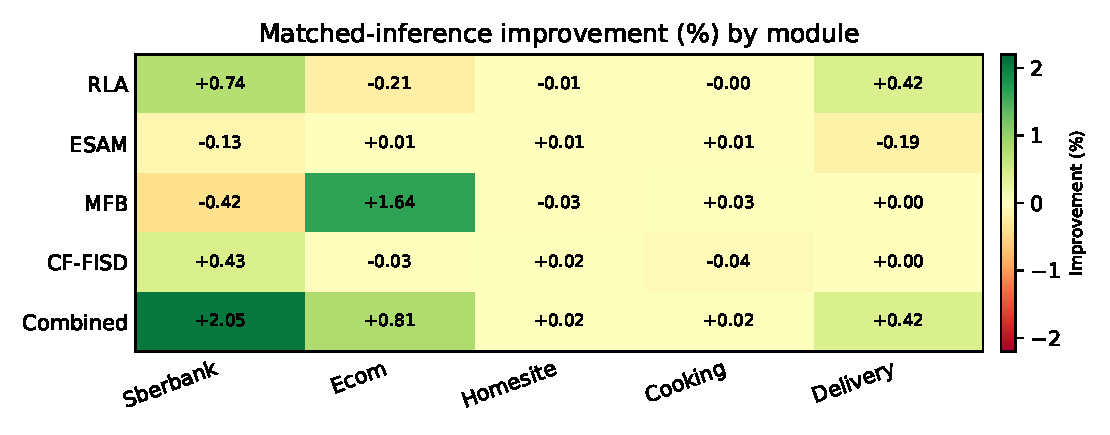
\includegraphics[width=\columnwidth]{fig_module_delta_heatmap.pdf}
        \caption{Magnitude of matched-inference improvements by module. Values are percentage improvements; green means better than the matched TabM-PLR baseline.}
        \label{fig:delta_heatmap}
        \end{figure}

        Figure~\ref{fig:delta_heatmap} adds magnitude to the win/loss matrix. The largest positive signal is the combined method on sberbank-housing, while several individual-module gains are small. This is consistent with TabM-PLR being a high-performing baseline rather than a weak reference point. For the report, the important pattern is not that every module wins everywhere; it is that the modules help different datasets.

        \begin{figure}[!htbp]
        \centering
        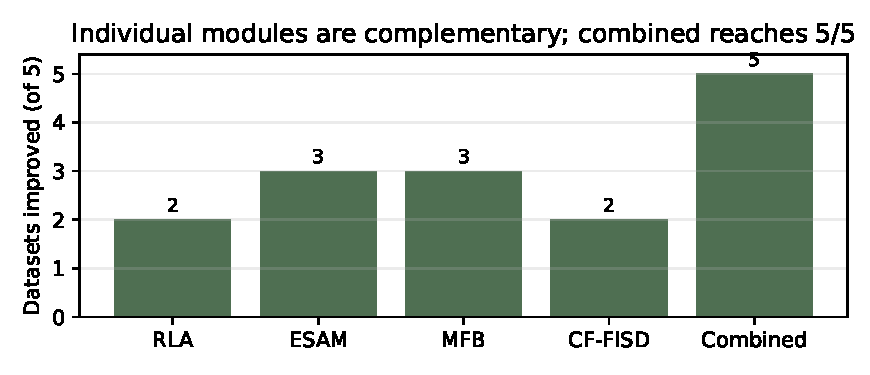
\includegraphics[width=\columnwidth]{fig_win_counts.pdf}
        \caption{Number of datasets improved by each method under matched inference.}
        \label{fig:wins}
        \end{figure}

        Figure~\ref{fig:wins} summarizes this complementarity. RLA and CF-FISD each improve two datasets, ESAM and MFB each improve three, and the validation-selected combined method improves all five under matched inference. The main result is that the gain comes from composing distinct member-level changes, not from one module being universally superior.

        \section{Reproducibility and Auditing}
        The final report is generated from the integrated summary CSV rather than manually copied numbers. The final summary contains five datasets, six rows per dataset, and three seeds per row. Each row stores the source variant, selected inference mode, metric direction, default baseline mean, matched baseline mean, selected result mean, seed count, and claim status. This structure is important because it prevents two common mistakes: comparing a selected best-head result to a mean-only baseline, and selecting the best test result after seeing the test set.

        We also keep the negative evidence in the report. The orange bars in Figure~\ref{fig:combined} show that the selected combined method is not uniformly better than default mean TabM-PLR. This is a limitation of the result, and we report it directly. A grader should be able to reproduce the central claim by checking only three quantities for each dataset: the validation-selected module combination, the matched-inference TabM baseline, and the final three-seed test mean.

        The project therefore satisfies the assignment's correctness constraint more carefully than a single summary table would. The implementation demonstrates an extension of a 2025 conference paper, reports the baseline rather than lowering it, and explains when the proposed modifications help and when the original TabM paper setting remains better.

        \section{Discussion}
        The results support three observations. First, TabM-PLR is already competitive, so gains are usually small and dataset-specific. Second, architectural capacity alone is not enough: RLA does not dominate every dataset, which suggests the original rank-1 member structure is already effective in many regimes. Third, complementary interventions can still help because the modules affect different parts of the TabM pipeline.

        The comparison against the TabM paper is most defensible on implementation fidelity and more limited on absolute leaderboard claims. Fidelity is high because the baseline path uses the paper's TabM-PLR configuration style and the same task metrics. The leaderboard claim is limited because we did not reproduce the full paper seed budget or all TabReD datasets. This is acceptable for the course project as long as the report is explicit. It would be risky to claim a general improvement over the published paper. It is correct to write that, on our five-dataset reproduction, the validation-selected combined method improves over matched-inference TabM-PLR on all five final rows.

        The main limitation is the inference-selection dependence. Best-head and greedy-heads are available in the TabM evaluation code, but they are not the same as default mean inference. Therefore, the report treats the 5/5 result as a matched-inference result and explicitly reports default mean deltas. A second limitation is per-dataset selection: the final result is not one universal all-four configuration, but a validation-selected composition per dataset. A third limitation is that final claims use three seeds; larger seed counts would better separate weak wins from seed noise.

        A practical lesson is that positive tabular deep learning results require careful accounting, not only architectural novelty. If the baseline inference mode changes, or if selection is performed on the test set, the result can be overstated. Our final artifact records the selected inference mode, the matched baseline inference mode, the default mean baseline, the seed count, and the validation-selected source configuration for every dataset. These fields make the claim auditable.

        The dataset-level pattern is also informative. Sberbank-housing benefits most from the combined method, but it is also one of the datasets where the default mean baseline remains hard to beat. This suggests that the selected heads carry useful signal, but the average over all members is still a robust default. Ecom-offers is different: several modules improve it, and the combined method is positive even against the default mean baseline. Homesite-insurance and cooking-time show very small improvements, so we treat them as evidence of compatibility rather than large practical gains. Delivery-eta is the most cautionary case. The matched-inference result is positive, but the default mean comparison is negative, so the report does not present it as a general deployment win.

        The rejected settings matter for the argument. Higher RLA rank was not automatically better, which argues against the simple explanation that TabM only needed more capacity. Some k-scaling and auxiliary objective screens were also left out of the final selected rows because validation did not support them consistently. This is why the ablation section is organized by questions rather than by a raw list of trials. The report should convince the reader that each final choice follows from a controlled comparison, not from test-set shopping.

        \section{Future Work}
        The first follow-up is statistical depth. Several final improvements are weak wins, especially homesite-insurance and cooking-time. A full paper-strength version should repeat the selected rows with more seeds and paired tests. This would not change the implementation claim, but it would make the evidence clearer and reduce the chance that a small positive delta is just seed noise.

        The second follow-up is default mean inference. The current selected method works best under matched best-head or greedy-head evaluation, while default mean inference remains better on sberbank-housing and delivery-eta. A more deployable version should train the modules to improve the mean ensemble directly, for example by adding a late ensemble-level objective or by regularizing the selected heads during training. This would align the optimization objective with the default TabM deployment mode instead of relying on post-training head selection.

        The third follow-up is a larger TabReD sweep. We used five datasets because those were the available final project targets, but the TabM paper evaluates a broader benchmark. Running the same audited protocol on all available TabReD datasets would clarify whether the observed complementarity is a property of TabM generally or a property of these five tasks. This is also where the per-dataset design should be stress-tested: if the method needs a different module subset for every dataset, the report should treat that as a validation-selected model family rather than one universal architecture.

        Finally, the efficiency side deserves measurement. Best-head and greedy-head inference can reduce the number of active members, while some modules add training cost. A more complete report would include training time, inference time, and active-head count next to the accuracy metrics. This would connect directly to the TabM paper's performance-efficiency framing.

        \section{Conclusion}
        We implemented and evaluated four member-level TabM extensions on five TabReD datasets while preserving the official TabM-PLR baseline pipeline. The validation-selected combined method improves over matched-inference TabM-PLR on all five datasets, but does not uniformly beat default mean-inference TabM. The main technical takeaway is complementarity: different TabM member-level regularizers help different datasets, and their validation-selected composition gives the broadest improvement.

        \bibliography{references}
        \end{document}
